\documentclass[polish]{beamer}
\usefonttheme[onlymath]{serif}
\usepackage[utf8]{inputenc}
\usepackage{silence}
\usepackage{polski}
%\usepackage[polish]{babel}
\usepackage{parskip}
\usepackage{amsmath,amsfonts,amssymb,amsthm}
\usepackage{mathtools}
%\usepackage{enumitem}
%\usepackage{pgfplots}
%\pgfplotsset{compat=1.16}
\usepackage{newunicodechar}
%\usepackage{etoolbox}
%\usepackage{algorithm}
%\usepackage{algorithmicx}
%\usepackage{algpseudocode}
\usepackage{bussproofs}
\usepackage{tikz}
\usepackage{listingsutf8}
\usepackage{cmll}
\usetikzlibrary{decorations.pathmorphing}
\setcounter{secnumdepth}{0}
\uselanguage{polish}
\languagepath{polish}

\title{Logika liniowa}
\author{Wiktor Kuchta}
\date{\today}

\DeclareMathOperator{\im}{Im}
\DeclareMathOperator{\rank}{rank}
\DeclareMathOperator{\Lin}{Lin}
\DeclareMathOperator{\sgn}{sgn}
\DeclareMathOperator{\Char}{char}
\newcommand{\N}{\mathbb{N}}
\newcommand{\Z}{\mathbb{Z}}
\newcommand{\Q}{\mathbb{Q}}
\newcommand{\R}{\mathbb{R}}
\newcommand{\C}{\mathbb{C}}
\newcommand{\inner}[2]{( #1 \, | \, #2)}
\newcommand{\norm}[1]{\left\lVert #1 \right\rVert}
\newcommand{\modulus}[1]{\left| #1 \right|}
\newcommand{\abs}{\modulus}
\newtheorem{lemat}{Lemat}
\newcommand{\ol}{\overline}
\DeclareMathOperator{\tr}{tr}
\DeclareMathOperator{\diag}{diag}
\newcommand{\+}{\enspace}
\newcommand{\sump}{\sideset{}{'}{∑}} % sum prime
\newcommand{\sumb}{\sideset{}{"}{∑}} % sum bis
\newcommand{\0}{\mathbf{0}}
\newcommand{\1}{\mathbf{1}}
\newcommand{\mb}{\multimapboth}
\usepackage{ulem}
\renewcommand<>{\sout}[1]{\alt#2{\beameroriginal{\sout}{#1}}{#1}}

\lstset{
	basicstyle=\ttfamily,
	columns=fullflexible,
	keepspaces=true
}

\DeclareRobustCommand{\&}{%
  \ifmmode\expandafter\mathbin\fi\char`&
}

\newunicodechar{∅}{\emptyset} % Digr /0
\newunicodechar{∞}{\infty} % Digr 00
\newunicodechar{∂}{\partial} % Digr dP
\newunicodechar{α}{\alpha}
\newunicodechar{β}{\beta}
\newunicodechar{ξ}{\xi} % Digr c*
\newunicodechar{δ}{\delta} % Digr d*
\newunicodechar{ε}{\varepsilon}
\newunicodechar{φ}{\varphi}
\newunicodechar{θ}{\theta} % Digr h*
\newunicodechar{λ}{\lambda}
\newunicodechar{μ}{\mu}
\newunicodechar{π}{\pi}
\newunicodechar{ψ}{\psi}
\newunicodechar{σ}{\sigma}
\newunicodechar{τ}{\tau}
\newunicodechar{ω}{\omega}
\newunicodechar{η}{\eta} % Digr y*
\newunicodechar{ζ}{\zeta} % Digr z*
\newunicodechar{Δ}{\Delta}
\newunicodechar{Γ}{\Gamma}
\newunicodechar{Λ}{\Lambda}
\newunicodechar{Θ}{\Theta}
\newunicodechar{Φ}{\Phi} % Digr F*
\newunicodechar{Π}{\Pi}
\newunicodechar{Ψ}{\Psi} % digr Q*
\newunicodechar{Σ}{\Sigma} % digr S*
\newunicodechar{Ω}{\Omega} % digr W*
\newunicodechar{ℕ}{\N} % Digr NN 8469 nonstandard
\newunicodechar{ℤ}{\Z} % Digr ZZ 8484 nonstandard
\newunicodechar{ℚ}{\Q} % Digr QQ 8474 nonstandard
\newunicodechar{ℝ}{\R} % Digr RR 8477 nonstandard
\newunicodechar{ℂ}{\C} % Digr CC 8450 nonstandard
\newunicodechar{∑}{\sum}
\newunicodechar{∏}{\prod}
\newunicodechar{∫}{\int}
\newunicodechar{∓}{\mp}
\newunicodechar{⌈}{\lceil} % Digr <7
\newunicodechar{⌉}{\rceil} % Digr >7
\newunicodechar{⌊}{\lfloor} % Digr 7<
\newunicodechar{⌋}{\rfloor} % Digr 7>
\newunicodechar{≅}{\cong} % Digr ?=
\newunicodechar{≡}{\equiv} % Digr 3=
\newunicodechar{◁}{\triangleleft} % Digr Tl
\newunicodechar{▷}{\triangleright} % Digr Tr
\newunicodechar{≤}{\le}
\newunicodechar{≥}{\ge}
\newunicodechar{≪}{\ll} % Digr <*
\newunicodechar{≫}{\gg} % Digr *>
\newunicodechar{≠}{\ne}
\newunicodechar{⊆}{\subseteq} % Digr (_
\newunicodechar{⊇}{\supseteq} % Digr _)
\newunicodechar{⊂}{\subset} % Digr (C
\newunicodechar{⊃}{\supset} % Digr C)
\newunicodechar{∩}{\cap} % Digr (U
\newunicodechar{∖}{\setminus} % Digr -\ nonstandard
\newunicodechar{∪}{\cup} % Digr )U
\newunicodechar{∼}{\sim} % Digr ?1
\newunicodechar{≈}{\approx} % Digr ?2
\newunicodechar{∈}{\in} % Digr (-
\newunicodechar{∋}{\ni} % Digr -)
\newunicodechar{∇}{\nabla} % Digr NB
\newunicodechar{∃}{\exists} % Digr TE
\newunicodechar{∀}{\forall} % Digr FA
\newunicodechar{∧}{\wedge} % Digr AN
\newunicodechar{∨}{\vee} % Digr OR
\newunicodechar{⊥}{\bot} % Digr -T
\newunicodechar{⊢}{\vdash} % Digr \- 8866 nonstandard
\newunicodechar{⊤}{\top} % Digr TO 8868 nonstandard
\newunicodechar{⇒}{\implies} % Digr =>
\newunicodechar{⊸}{\multimap} % Digr #> nonstandard
\newunicodechar{⇐}{\impliedby} % Digr <=
\newunicodechar{⇔}{\iff} % Digr ==
\newunicodechar{↔}{\leftrightarrow} % Digr <>
\newunicodechar{↦}{\mapsto} % Digr T> 8614 nonstandard
\newunicodechar{∘}{\circ} % Digr Ob
\newunicodechar{⊕}{\oplus} % Digr O+ 8853
\newunicodechar{⊗}{\otimes} % Digr OX 8855
\newunicodechar{⅋}{\parr}

% cursed
\WarningFilter{newunicodechar}{Redefining Unicode}
\newunicodechar{·}{\ifmmode\cdot\else\textperiodcentered\fi} % Digr .M
\newunicodechar{×}{\ifmmode\times\else\texttimes\fi} % Digr *X
\newunicodechar{→}{\ifmmode\rightarrow\else\textrightarrow\fi} % Digr ->
\newunicodechar{←}{\ifmmode\leftarrow\else\textleftarrow\fi} % Digr ->
\newunicodechar{⟨}{\ifmmode\langle\else\textlangle\fi} % Digr LA 10216 nonstandard
\newunicodechar{⟩}{\ifmmode\rangle\else\textrangle\fi} % Digr RA 10217 nonstandard
\newunicodechar{…}{\ifmmode\dots\else\textellipsis\fi} % Digr .,
\newunicodechar{±}{\ifmmode\pm\else\textpm\fi} % Digr +-


\begin{document}

\frame{\titlepage}

\section[intro]{Wstęp}

\begin{frame}
	\frametitle{Główna idea}
	Logika liniowa to logika substrukturalna pozbawiona reguł
	\begin{center}
		osłabienia (\textit{weakening})
		\hskip 1em
		\AxiomC{$Γ ⊢ Σ$}
		\UnaryInfC{$Γ, A ⊢ Σ$}
		\DisplayProof
		\hskip 1em
		\AxiomC{$Γ ⊢ Σ$}
		\UnaryInfC{$Γ ⊢ Σ, A$}
		\DisplayProof
	\end{center}
	\begin{center}
		i skracania (\textit{contraction}).
		\hskip 1em
		\AxiomC{$Γ, A, A ⊢ Σ$}
		\UnaryInfC{$Γ, A ⊢ Σ$}
		\DisplayProof
		\hskip 1em
		\AxiomC{$Γ ⊢ A, A, Σ$}
		\UnaryInfC{$Γ ⊢ A, Σ $}
		\DisplayProof
	\end{center}
	Poprzedniki sekwentów możemy interpretować jako zasoby
	(\textit{resources}), których nie możemy brać znikąd i marnować.
\end{frame}

\begin{frame}
	\frametitle{Kontekst historyczny}
	Logikę liniową wprowadził Jean-Yves Girard w 1987.
	Do odkrycia doprowadziło go studiowanie
	przestrzeni zgodności $(\textit{coherence spaces})$,
	które mogą stanowić semantykę programów liniowych i
	mają pewne podobieństwa z przestrzeniami liniowymi.

	% zaczął z językiem funkcyjnym/systemem dowodów, potem sformułował logikę

	% system F, który jest podstawą np. Haskella i OCamla
	% paradoks Girarda w systemie U
	% zegarki z musztardą

	% logika afiniczna (bez skracania) została wprowadzona już w 1974
	% prace nad różnymi relevant logics się zaczęły ok. 50 lat wcześniej

\end{frame}

\begin{frame}
	\frametitle{Reguły addytywne i multiplikatywne}
	W klasycznym rachunku sekwentów reguły możemy zaprezentować
	w sposób \textit{addytywny}:

	\vskip 1em

	\begin{center}
		\AxiomC{$Γ, φ_i ⊢ Σ$}
		\RightLabel{$∧$L$_i$}
		\UnaryInfC{$Γ, φ_1 ∧ φ_2 ⊢ Σ$}
		\DisplayProof
		\hskip 1em
		\AxiomC{$Γ ⊢ φ_1, Σ$}
		\AxiomC{$Γ ⊢ φ_2, Σ$}
		\RightLabel{$∧$R}
		\BinaryInfC{$Γ ⊢ φ_1 ∧ φ_2, Σ$}
		\DisplayProof
	\end{center}
	\vskip 1em
	albo \textit{multiplikatywny}:
	\vskip 1em
	\begin{center}
		\AxiomC{$Γ, φ_1, φ_2 ⊢ Σ$}
		\RightLabel{$∧$L}
		\UnaryInfC{$Γ, φ_1 ∧ φ_2 ⊢ Σ$}
		\DisplayProof
		\hskip 1em
		\AxiomC{$Γ_1 ⊢ φ_1, Σ_1$}
		\AxiomC{$Γ_2 ⊢ φ_2, Σ_2$}
		\RightLabel{$∧$R}
		\BinaryInfC{$Γ_1, Γ_2 ⊢ φ_1 ∧ φ_2, Σ_1, Σ_2$}
		\DisplayProof
	\end{center}

	% w regułach multiplikatywnych,
	% wszystkie zmienne w konkluzji pojawiają się dokładnie raz w przesłankach

	% Dlaczego równoważne?
	% ⊕ to lower bound, ⊗ to przecinek
\end{frame}

\begin{frame}
	Girard zauważył, że reguły strukturalne są powiązane z niekonstruktywnością logiki klasycznej.

	\textbf{Przykład:} W intuicjonistycznym rachunku sekwentów łatwo pokazać,
	że jeśli $⊢ A ∨ B$, to $⊢ A$ lub $⊢ B$.
	Korzystamy z tego, że jedyna pasująca reguła to wprowadzenie alternatywy.
	W rachunku klasycznym mogło dojść do skracania po prawej.

	\textbf{Przykład:} Dowodzimy nie wprost $∃x. \, P(x)$, czyli zakładamy $∀x. \lnot P(x)$.
	Aby skorzystać z założenia, musimy podać jakiegoś konkretnego $x_1$.
	Jeśli wtedy dojdziemy do sprzeczności, to znaleźliśmy $x$, dla którego $\lnot \lnot P(x) ≡ P(x)$.
	Dopiero kiedy skorzystamy z założenia \textit{wielokrotnie},
	to nie możemy wskazać konkretnego takiego $x$.

	% skracanie jest większym winowajcą
	% logika ze osłabianiem, ale bez skracania — afiniczna (affine)
\end{frame}

\section[sekwenty]{Liniowy rachunek sekwentów}

\begin{frame}
	\frametitle{Koniunkcja addytywna}
	Czytamy $A$ \textit{wraz z} $B$ ($A$ \textit{with} $B$).
	\begin{center}
		\AxiomC{$Γ, φ_i ⊢ Σ$}
		\RightLabel{$\&$L$_i$}
		\UnaryInfC{$Γ, φ_1\& φ_2 ⊢ Σ$}
		\DisplayProof
		\hskip 1em
		\AxiomC{$Γ ⊢ φ_1, Π$}
		\AxiomC{$Γ ⊢ φ_2, Π$}
		\RightLabel{$\&$R}
		\BinaryInfC{$Γ ⊢ φ_1 \& φ_2, Π$}
		\DisplayProof
	\end{center}
	\vskip 1em
	Element neutralny to \textit{top}:
	\begin{center}
		\AxiomC{}
		\RightLabel{$⊤$R}
		\UnaryInfC{$Γ ⊢ ⊤, Σ$}
		\DisplayProof
	\end{center}
	% Intuicja: jak mamy A & B, to umiemy udowodnić i A i B,
	% ale musimy wybrać tylko jedno z nich.
\end{frame}

\begin{frame}
	\frametitle{Koniunkcja multiplikatywna}
	%\tableofcontents[currentsection]
	Czytamy $A$ \textit{tensor} $B$ lub $A$ \textit{i} $B$.
	\begin{center}
		\AxiomC{$Γ, φ_1, φ_2 ⊢ Σ$}
		\RightLabel{$⊗$L}
		\UnaryInfC{$Γ, φ_1 ⊗ φ_2 ⊢ Σ$} % zamienia przecinek na tensor
		\DisplayProof
		\hskip 1em
		\AxiomC{$Γ_1 ⊢ φ_1, Σ_1$}
		\AxiomC{$Γ_2 ⊢ φ_2, Σ_2$}
		\RightLabel{$⊗$R}
		\BinaryInfC{$Γ_1, Γ_2 ⊢ φ_1 ⊗ φ_2, Σ_1, Σ_2$}
		\DisplayProof
	\end{center}
	\vskip 1em
	Element neutralny to jedynka (\textit{unit}):
	\begin{center}
		\AxiomC{$Γ ⊢ Σ$}
		\RightLabel{$1$L}
		\UnaryInfC{$Γ, 1 ⊢ Σ$}
		\DisplayProof
		\hskip 1em
		\AxiomC{}
		\RightLabel{$1$R}
		\UnaryInfC{$⊢ 1$}
		\DisplayProof
	\end{center}
	% po prostu para
\end{frame}

\begin{frame}
	\frametitle{Alternatywa addytywna}
	%\tableofcontents[currentsection]
	Czytamy $A$ \textit{plus} $B$.
	\begin{center}
		\AxiomC{$Γ, φ_1 ⊢ Σ$}
		\AxiomC{$Γ, φ_2 ⊢ Σ$}
		\RightLabel{$⊕$L}
		\BinaryInfC{$Γ, φ_1 ⊕ φ_2 ⊢ Σ$}
		\DisplayProof
		\hskip 1em
		\AxiomC{$Γ ⊢ φ_i, Σ$}
		\RightLabel{$⊕$R$_i$}
		\UnaryInfC{$Γ ⊢ φ_1 ⊕ φ_2, Σ$}
		\DisplayProof
	\end{center}
	\vskip 1em
	Element neutralny to zero:
	\begin{center}
		\AxiomC{}
		\RightLabel{$0$L}
		\UnaryInfC{$Γ, 0 ⊢ Σ$}
		\DisplayProof
	\end{center}
\end{frame}

\begin{frame}
	\frametitle{Alternatywa multiplikatywna}
	Czytamy $A$ \textit{par} $B$.
	\begin{center}
		\AxiomC{$Γ_1, φ_1 ⊢ Σ_1$}
		\AxiomC{$Γ_2, φ_2 ⊢ Σ_2$}
		\RightLabel{$⅋$L}
		\BinaryInfC{$Γ_1, Γ_2, φ_1 ⅋ φ_2 ⊢ Σ_1, Σ_2$}
		\DisplayProof
		\hskip 1em
		\AxiomC{$Γ ⊢ φ_1, φ_2, Σ$}
		\RightLabel{$⅋$R}
		\UnaryInfC{$Γ ⊢ φ_1 ⅋ φ_2, Σ$}
		\DisplayProof
	\end{center}
	\vskip 1em
	Element neutralny to \textit{bottom}:
	\begin{center}
		\AxiomC{}
		\RightLabel{$⊥$L}
		\UnaryInfC{$⊥ ⊢$}
		\DisplayProof
		\hskip 1em
		\AxiomC{$Γ ⊢ Σ$}
		\RightLabel{$⊥$R}
		\UnaryInfC{$Γ ⊢ Σ, ⊥$}
		\DisplayProof
	\end{center}

\end{frame}

\begin{frame}
	\frametitle{Negacja i liniowa implikacja}
	\begin{center}
		\AxiomC{$Γ ⊢ φ, Σ$}
		\RightLabel{$^⊥$L}
		\UnaryInfC{$Γ, φ^⊥ ⊢ Σ$}
		\DisplayProof
		\hskip 1em
		\AxiomC{$Γ, φ ⊢ Σ$}
		\RightLabel{$^⊥$R}
		\UnaryInfC{$Γ ⊢ φ^⊥ , Σ$}
		\DisplayProof
	\end{center}
	\vskip 1em
	Czasami czytamy $A$ \textit{lizak} $B$ (\textit{lolli}, \textit{lollipop}).
	\begin{center}
		\AxiomC{$Γ_1 ⊢ φ, Σ_1$}
		\AxiomC{$Γ_2, ψ ⊢ Σ_2$}
		\RightLabel{$⊸$L}
		\BinaryInfC{$Γ_1, Γ_2, φ ⊸ ψ ⊢ Σ_1, Σ_2$}
		\DisplayProof
		\hskip 1em
		\AxiomC{$Γ, φ ⊢ ψ, Σ$}
		\RightLabel{$⊸$R}
		\UnaryInfC{$Γ ⊢ φ ⊸ ψ, Σ$}
		\DisplayProof
		%reguły takie same jak dla zwykłe implikacji
	\end{center}
	\vskip 1em
	\textit{Równoważność} $A \multimapboth B$ definiujemy jako
	$(A ⊸ B) \& (B ⊸ A)$.
	Mamy $Γ ⊢ A \multimapboth B$ wtedy i tylko wtedy, gdy
	$Γ ⊢ A ⊸ B$ i $Γ ⊢ B ⊸ A$.

	Zachodzi $(A ⊸ B) \multimapboth A^⊥ ⅋ B$.

\end{frame}

\begin{frame}
	\frametitle{Menu}
	\begin{align*}10 \textrm{ zł}
		\multimap & (\textit{pomidorowa} \with \textit{krupnik}) \\
		⊗& (\textit{kotlet} \with \textit{ryba}) \\
		⊗& (\textit{kompot jabłkowy} ⊕ \textit{kompot śliwkowy})
	\end{align*}
\end{frame}

\begin{frame}
	\frametitle{Symetria}
	Lewą regułę spójnika możemy porównać z prawą regułą spójnika dualnego,
	na przykład:
	\begin{center}
		\AxiomC{$Γ, φ_i ⊢ Σ$}
		\RightLabel{$\&$L$_i$}
		\UnaryInfC{$Γ, φ_1\& φ_2 ⊢ Σ$}
		\DisplayProof
		\hskip 1em
		\AxiomC{$Γ ⊢ φ_i, Σ$}
		\RightLabel{$⊕$R$_i$}
		\UnaryInfC{$Γ ⊢ φ_1 ⊕ φ_2, Σ$}
		\DisplayProof
	\end{center}
	% prawie de morgan (negacja przestawia strony sekwentu)
\end{frame}

\begin{frame}
	\frametitle{Prawa de Morgana}
	$$A \multimapboth A^{⊥⊥}$$

	\begin{equation*}
	\begin{split}
	(A ⊗ B)^⊥ &\mb A^⊥ ⅋ B^⊥ \\
	1^⊥ &\mb ⊥ \\
	(A ⊕ B)^⊥ &\mb A^⊥ \with B^⊥ \\
	0^⊥ &\mb ⊤
	\end{split}
	\quad \quad \quad
	\begin{split}
	(A ⅋ B)^⊥ &\mb A^⊥ ⊗ B^⊥ \\
	⊥^⊥ &\mb 1 \\
	(A \with B)^⊥ &\mb A^⊥ ⊕ B^⊥ \\
	T^⊥ &\mb 0
	\end{split}
	\end{equation*}
	% w liniowej spójniki są definiowalne za pomocą innych, co nie zachodzi w intui
\end{frame}

\begin{frame}
	\frametitle{Rozdzielność ,,mnożenia'' względem ,,dodawania''}
	$$A ⊗ (B ⊕ C) \mb (A ⊗ B) ⊕ (A ⊗ C)$$
	$$A ⅋ (B \& C) \mb (A ⅋ B) \& (A ⅋ C)$$
	$$0 \mb A ⊗ 0$$
	$$⊤ \mb A ⅋ ⊤$$
	% i analogicznie kiedy spójnik multiplikatywny będzie po prawej
\end{frame}

\begin{frame}
	\frametitle{Kontrolowane użycie reguł strukturalnych}
	$\oc A$ (\textit{oczywiście} $A$) i $\wn A$ (\textit{być może} $A$) pozwalają
	na kontrolowane użycie reguł strukturalnych.
	\begin{center}
		\AxiomC{$Γ, φ ⊢ Σ$}
		\RightLabel{$\oc $L}
		\UnaryInfC{$Γ, \oc φ ⊢ Σ$}
		\DisplayProof
		\hskip 1em
		\AxiomC{$\oc Γ ⊢ φ, \wn Σ$}
		\RightLabel{$\oc $R}
		\UnaryInfC{$\oc Γ ⊢ \oc φ, \wn Σ$}
		\DisplayProof
	\end{center}
	\begin{center}
		\AxiomC{$\oc Γ , φ ⊢ \wn Σ$}
		\RightLabel{$\wn $L}
		\UnaryInfC{$\oc Γ, \wn φ ⊢ \wn Σ$}
		\DisplayProof
		\hskip 1em
		\AxiomC{$Γ ⊢ φ, Σ$}
		\RightLabel{$\wn $R}
		\UnaryInfC{$Γ ⊢ \wn φ, Σ$}
		\DisplayProof
	\end{center}

	\begin{center}
		\AxiomC{$Γ ⊢ Σ$}
		\RightLabel{$\oc $W}
		\UnaryInfC{$Γ, \oc φ ⊢ Σ$}
		\DisplayProof
		\hskip 1em
		\AxiomC{$Γ, \oc φ, \oc φ ⊢ Σ$}
		\RightLabel{$\oc $C}
		\UnaryInfC{$Γ, \oc φ ⊢ Σ$}
		\DisplayProof
	\end{center}

	\begin{center}
		\AxiomC{$Γ ⊢ Σ$}
		\RightLabel{$\wn $W}
		\UnaryInfC{$Γ ⊢ \wn φ, Σ$}
		\DisplayProof
		\hskip 1em
		\AxiomC{$Γ ⊢ \wn  φ, \wn  φ, Σ$}
		\RightLabel{$\wn  $C}
		\UnaryInfC{$Γ ⊢ \wn  φ, Σ$}
		\DisplayProof
	\end{center}
	Intuicyjnie, $\oc A$ może wyprodukować dowolną liczbę $A$,
	a $\wn A$ pewną liczbę $A$.


	% teraz w menu możemy wpisać nieograniczone dolewki kawy
\end{frame}

\begin{frame}
	\frametitle{Operatory wykładnicze}
	Nazwa wynika z $\oc(A \& B) \mb \oc A ⊗ \oc B$ i $\wn(A ⊕ B) \mb \wn A ⅋ \wn B$.
	$$(\oc  A)^⊥ \mb \wn (A^⊥)$$
	$$(\wn  A)^⊥ \mb \oc (A^⊥)$$

	\vskip 1em
	$$\oc A ≈ 1 \& A \& (A ⊗ A) \& (A ⊗ A ⊗ A) \& …$$
	$$\wn A ≈ ⊥ ⊕ A ⊕ (A ⅋ A) ⊕ (A ⅋ A ⅋ A) ⊕ …$$

\end{frame}

\begin{frame}
	\frametitle{Translacja Girarda}
	Jest możliwych kilka translacji z logiki intuicjonisticznej zachowujących dowodliwość,
	np.
	\begin{align*}
		Φ(A ⇒ B) &= \oc Φ(A) ⊸ Φ(B) \\
		Φ(A ∧ B) &= \oc Φ(A) \with \oc Φ(B) \\
		Φ(T) &= ⊤ \\
		Φ(F) &= 0 \\
		Φ(A ∨ B) &= \oc Φ(A) ⊕ \oc Φ(B) \\
		Φ(Γ ⊢ A) &= \oc Φ(Γ) ⊢ Φ(A)
	\end{align*}

	Możemy to złożyć z translacją logiki klasycznej w intuicjonistyczną,
	otrzymując włożenie logiki klasycznej w liniową.
\end{frame}

\begin{frame}
	\frametitle{Cięcie}
	\begin{center}
		\AxiomC{$Γ ⊢ φ, Σ$}
		\AxiomC{$Δ, φ ⊢ Π$}
		\RightLabel{Cut}
		\BinaryInfC{$Γ,Δ ⊢ Σ, Π$}
		\DisplayProof
	\end{center}
	\begin{theorem}Jeśli sekwent ma dowód, to ma dowód bez cięcia.
	\end{theorem}
	% Łatwo wywnioskować niesprzeczność
	\begin{theorem}W dowodzie bez cięcia dla sekwentu $⊢ Γ$ występują wyłącznie podformuły formuł z $Γ$.
	\end{theorem}
	\begin{theorem}
		Jeśli $⊢ A ⊗ B$ to $⊢ A$ i $⊢ B$.
		Jeśli $⊢ A ⊕ B$ to $⊢ A$ lub $⊢ B$.
	\end{theorem}
\end{frame}

\section[seman]{Semantyki logiki liniowej}

\begin{frame}
	\frametitle{Semantyki logiki liniowej}
	\begin{itemize}
		\item przestrzenie zgodności
		\item semantyka fazowa  % semantyka formuł, a nie dowodów
		\item semantyka kategoryjna
		\item semantyka relacyjna
		\item geometria interakcji
		\item semantyka w teorii gier
			% formuła interpretujemy jako grę dwóch graczy
			% stałe multiplikatywne kończą grę
			% stałe addytywne kończą ruchy, gra trwa w nieskończoność
			% stałe koniunktywne wygrywamy
			% stałe alternatywne przegrywamy
			% w koniunkcji oni wybierają grę, kto ma kontrole musi wygrać co najmniej jedną
			% w dodawaniu wybiera się grę, w mnożeniu mamy dwie gry równolegle
	\end{itemize}
\end{frame}

%\begin{frame} \frametitle{Semantyka fazowa} \end{frame}

\begin{frame}
	\frametitle{Intuicjonizm i interpretacja BHK}
	Z logiką intuicjonistyczną jest kojarzona interpretacja Brouwera-Heytinga-Kołmogorowa,
	która mówi, że znaczeniem formuły jest jej dowód,
	a dowodem jest pewien obiekt matematyczny.

	W intuicjonizmie za pojęcia pierwotne bierzemy prawdę i absurd,
	negacja jest pojęciem wtórnym.
	Czasami mamy do czynienia z bardziej naturalnym pojęciem fałszu niż dojściem do absurdu.

\end{frame}

\begin{frame}
	\frametitle{Interpretacja z tezami i antytezami}
	Formułę zrozumiemy, kiedy zrozumiemy, co się liczy jako jej dowód i co się liczy jako jej zaprzeczenie.

	Przykłady:

	Dowodem $A ⊕ B$ jest para dowodów $A$ i $B$.
	Zaprzeczeniem $A ⊕ B$ jest zaprzeczenie $A$ lub zaprzeczenie $B$.

	Dowodem $A ⊗ B$ jest para dowodów $A$ i $B$.
	Zaprzeczeniem $A ⊗ B$ jest sposób przekształcania dowodów $A$ na zaprzeczenia $B$ i dowodów $B$ na zaprzeczenia $A$.
\end{frame}

\begin{frame}
	\frametitle{\textit{Linear logic for constructive mathematics}}
	W matematyce konstruktywnej rozważane są często pary $P^+$ i $P^-$,
	które są swoimi negacjami klasycznie,
	ale nie intuicjonistycznie, np.
	$$∃q ∈ ℚ, x = q$$
	$$∀q ∈ ℚ, x \# q$$
	W 2018 M. Shulman odkrył, że takie pary można automatycznie znaleźć
	interpretując ,,naturalnie'' odpowiadające pojęciu zdanie logiki liniowej
	w logice intuicjonistycznej.
\end{frame}


\section[intuit]{Intuicjonistyczna logika liniowa}
\begin{frame}
	\frametitle{Modelowanie stanu}
	\begin{center}
	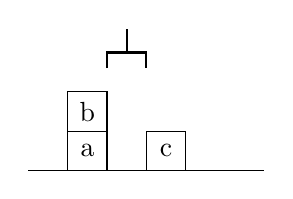
\begin{tikzpicture}
		\draw (0, 0) -- (3,0);
		\draw (0.5,0) rectangle (1,0.5) node[midway] {a};
		\draw (0.5,0.5) rectangle (1,1) node[midway] {b};
		\draw (1.5,0) rectangle (2,0.5) node[midway] {c};
		\draw [thick] (1,1.3) -- (1,1.5) -- (1.5, 1.5) -- (1.5, 1.3);
		\draw [thick] (1.25, 1.5) -- (1.25, 1.8);
	\end{tikzpicture}
	\end{center}
	$$Γ_0 = \{ \mathrm{empty}, \mathrm{tbl}(a), \mathrm{on}(b,a), \mathrm{clear}(b), \mathrm{tbl}(c), \mathrm{clear}(c) \}$$
	Jak zakodować ,,jeśli chwytak robota jest pusty i na bloku $x$ nic nie ma i blok $x$ leży na $y$,
	to robot może podnieść $x$, wtedy $x$ jest w chwytaku, a na $y$ nic nie ma''?
$$∀x. \, ∀y.\, \mathrm{empty} ∧ \mathrm{clear}(x) ∧ \mathrm{on}(x,y) ⇒ \mathrm{holds}(x) ∧ \mathrm{clear}(y)$$
$$∀x. \, ∀y.\, \mathrm{empty} ∧ \mathrm{clear}(x) ∧ \mathrm{on}(x,y) ⇒ \bigcirc(\mathrm{holds}(x) ∧ \mathrm{clear}(y))$$
$$∀x. \, ∀y.\, \mathrm{empty} ⊗ \mathrm{clear}(x) ⊗ \mathrm{on}(x,y) ⊸ \mathrm{holds}(x) ⊗ \mathrm{clear}(y)$$
\end{frame}

\begin{frame}
	\frametitle{Intuicjonistyczna logika liniowa}
	Podobnie jak z klasycznym rachunkiem sekwentów, aby otrzymać intuicjonistyczny
	odpowiednik, zabraniamy mieć więcej niż jedną formułę po prawej stronie sekwentu.
	Wtedy tracą sens spójniki $⅋, \wn, ^⊥, ⊥$.

	Istnieje także intuicjonistyczna liniowa dedukcja naturalna,
	której reguły lepiej odzwierciedlają obliczeniowy sens spójników.

\end{frame}

\begin{frame}

	\begin{center}
		\AxiomC{$Δ ⊢ A$}
		\AxiomC{$Δ' ⊢ B$}
		\RightLabel{$⊗$I}
		\BinaryInfC{$Δ, Δ' ⊢ A ⊗ B$}
		\DisplayProof
		\hskip 1em
		\AxiomC{$Δ ⊢ A ⊗ B$}
		\AxiomC{$Δ', A, B ⊢ C$}
		\RightLabel{$⊗$E}
		\BinaryInfC{$Δ, Δ' ⊢ C$}
		\DisplayProof
	\end{center}
	\vskip 1em

	\begin{center}
		\AxiomC{$Δ ⊢ A$}
		\AxiomC{$Δ ⊢ B$}
		\RightLabel{$\&$I}
		\BinaryInfC{$Δ ⊢ A \& B$}
		\DisplayProof
		\hskip 1em
		\AxiomC{$Δ ⊢ A \& B$}
		\RightLabel{$\&$E\textsubscript{L}}
		\UnaryInfC{$Δ ⊢ A$}
		\DisplayProof
		\hskip 1em
		\AxiomC{$Δ ⊢ A \& B$}
		\RightLabel{$\&$E\textsubscript{R}}
		\UnaryInfC{$Δ ⊢ B$}
		\DisplayProof
	\end{center}
	\vskip 1em
	\begin{center}
		\AxiomC{$Δ, A ⊢ B$}
		\RightLabel{$⊸$I}
		\UnaryInfC{$Δ ⊢ A ⊸ B$}
		\DisplayProof
		\hskip 1em
		\AxiomC{$Δ ⊢ A ⊸ B$}
		\AxiomC{$Δ' ⊢ A$}
		\RightLabel{$⊸$E}
		\BinaryInfC{$Δ ⊢ A$}
		\DisplayProof
	\end{center}
	\vskip 1em
	\begin{center}
		\AxiomC{}
		\RightLabel{$1$I}
		\UnaryInfC{$· ⊢ 1$}
		\DisplayProof
		\hskip 1em
		\AxiomC{$Δ ⊢ 1$}
		\AxiomC{$Δ' ⊢ C$}
		\RightLabel{$1$E}
		\BinaryInfC{$Δ, Δ' ⊢ C$}
		\DisplayProof
	\end{center}
	\vskip 1em
	\begin{center}
		\AxiomC{$Δ ⊢ 0$}
		\RightLabel{$0$E}
		\UnaryInfC{$Δ, Δ' ⊢ C$}
		\DisplayProof
		\hskip 1em
		\AxiomC{}
		\RightLabel{$⊤$I}
		\UnaryInfC{$Δ ⊢ ⊤$}
		\DisplayProof
	\end{center}

	\vskip 1em
	\begin{center}
		\AxiomC{$Δ ⊢ A$}
		\RightLabel{$⊕$I\textsubscript{L}}
		\UnaryInfC{$Δ ⊢ A ⊕ B$}
		\DisplayProof
		\hskip 1em
		\AxiomC{$Δ ⊢ B$}
		\RightLabel{$⊕$I\textsubscript{R}}
		\UnaryInfC{$Δ ⊢ A ⊕ B$}
		\DisplayProof

		\vskip 1em

		\AxiomC{$Δ ⊢ A ⊕ B$}
		\AxiomC{$Δ, A ⊢ C$}
		\AxiomC{$Δ, B ⊢ C$}
		\RightLabel{$⊕$E}
		\TrinaryInfC{$Δ, Δ' ⊢ C$}
		\DisplayProof
	\end{center}
\end{frame}

\begin{frame}
	\frametitle{Zasoby w programowaniu}
	Co traktujemy jako zasoby, z którymi musimy się ostrożnie obchodzić?
	To zależy. Na przykład

	\begin{enumerate}
		\item deskryptory plików
		\item sockety
		\item obszary pamięci programu
		\item obszary pamięci innego programu/urządzenia?
	\end{enumerate}
	% zasoby reprezentowalne jako jakaś wartość w języku
	% zasoby niereprezentowalne np czas CPU
\end{frame}

\begin{frame}[fragile]
	\frametitle{Konstrukcje językowe do zarządzania zasobami}
	Wiele języków ma specjalne konstrukcje do sprzątania po zasobach,
	np. \texttt{try/finally}, \texttt{with}, \texttt{UNWIND-PROTECT}...

\begin{onlyenv}<1>
	\begin{lstlisting}

with open(filename) as file_handle:
    ...
	\end{lstlisting}
\end{onlyenv}
\begin{onlyenv}<2->
	\begin{lstlisting}
foo = None
with open(filename) as file_handle:
    foo = file_handle
print(foo.read())

... ValueError: I/O operation on closed file.
	\end{lstlisting}
\end{onlyenv}
\end{frame}

\begin{frame}
	\frametitle{Linear Haskell}
	Co to znaczy użyć wartość? Czy można mówić o gwarantowanym użyciu wartości
	w języku leniwym, z wyjątkami i nieskończonymi pętlami?

	W Linear Haskellu $\mathtt{f :: A ⊸ B}$ gwarantuje,
	że jeśli $\mathtt{(f\+x)}$ jest użyte dokładnie raz,
	to $\mathtt{f}$ użyła $\mathtt{x}$ dokładnie raz, gdzie
	\begin{enumerate}
		\item aby użyć wartość prymitywnego typu (np. \texttt{Int}),
			po prostu ją trzeba zewaluować
		\item aby użyć funkcję, stosujemy ją do argumentu i wynik używamy dokładnie raz
		\item aby użyć parę, używamy oba komponenty pary dokładnie raz
		\item aby użyć wartość algebraicznego typu danych,
			robimy pattern matching wszystkich konstruktorów i
			w każdym przypadku pola liniowe używamy dokładnie raz
	\end{enumerate}
\end{frame}

\begin{frame}
	$\mathtt{data\+ a ⊗ b = Pair\+a\+b}$ \\
	$\mathtt{data\+ a ⊕ b = Left\+a \mid Right\+b}$ \\
	$\mathtt{type\+ a \& b = ∀r.\+ ((a ⊸ r) ⊕ (b ⊸ r)) ⊸ r}$ \\
	$\mathtt{data\+ \oc a \+where\+\{ Ur :: a → \oc a \}}$
	\vskip 1em
	$\mathtt{id :: a ⊸ a}$ \\
	$\mathtt{id\+x = x}$
	\vskip 1em
	$\mathtt{fst :: a ⊗ b → a}$ \\
	$\mathtt{fst\+(Pair\+a\+b) = a}$

\end{frame}

\begin{frame}
	\begin{center}
		\textit{Linearity} \\
		$⇒$ wartość nie będzie duplikowana \\
		\vskip 1em
		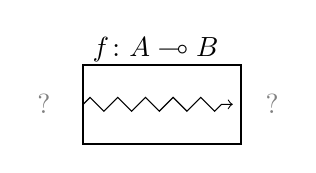
\begin{tikzpicture}
			\node[text width=50] at (0,0.7) {$f\colon A \multimap B$};
			\draw[black, thick] (-1,-0.5) rectangle (1,0.5);
			\node<1->[text width=5, align=center] at (-1.5,0) {\textcolor{gray}{?}};
			\node<1->[text width=5, align=center] at (1.4,0) {\textcolor{gray}{?}};
			\draw[->, thin, decorate, decoration={zigzag}] (-1,0) -- (0.9, 0);
		\end{tikzpicture}
	\end{center}

	\vskip 3em

	\begin{center}
		\textit{Uniqueness} \\
		$⇒$ wartość nie była wcześniej duplikowana \\
		\vskip 1em
		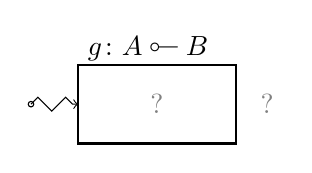
\begin{tikzpicture}
			\node[text width=50] at (0,0.7) {$g\colon A \mathbin{\rotatebox[origin=c]{-180}{$\multimap$}} B$};
			\draw[black, thick] (-1,-0.5) rectangle (1,0.5);
			\node<1->[text width=5, align=center] at (0,0) {\textcolor{gray}{?}};
			\node<1->[text width=5, align=center] at (1.4,0) {\textcolor{gray}{?}};
			\draw[->, thin, decorate, decoration={zigzag}] (-1.6,0) -- (-1, 0);
			\draw (-1.6,0) circle (1pt);
		\end{tikzpicture}
	\end{center}
\end{frame}
\begin{frame}
	Co nam mogą dać liniowość i unikalne referencje gwarantowane przez system typów?

	\textit{Linearity}
	\begin{enumerate}
		\item liniową funkcję można agresywnie inlinować
		\item typy nam więcej mówią, np. $[a] ⊸ [a]$ to permutacja listy
		\item liniowe użycie strumieni danych pozwala na przewidywalną optymalizację \textit{fusion}
	\end{enumerate}
	\textit{Uniqueness}
	\begin{enumerate}
		\item unikalny dostęp do danych pozwala je bezpiecznie modyfikować w miejscu
		\item unikalne referencje mają statycznie wyznaczony czas życia -- nie potrzebują garbage collectora
	\end{enumerate}
\end{frame}

\begin{frame}%[fragile]
	Jeśli chcemy stworzyć typ $T$, do którego referencje są zawsze unikalne, to
	możemy schować konstrukcję $T$ za interfejsem, który przyjmuje liniową
	kontynuację konsumującą $T$:
	$$∀r.\, (T ⊸ \oc r) ⊸ r$$
	Do tej kontynuacji musimy podawać świeżo skonstruowane wartości $T$.

	Przykład z Haskella:

	$\mathtt{alloc :: ∀a\,b.\,Int → a → (Array\,a ⊸ \oc b) ⊸ b}$ \\
	$\mathtt{toList :: ∀a.\,Array\,a ⊸ \oc [a]}$ \\
	$\mathtt{set :: ∀a.\,Int → a → Array\,a ⊸ Array\,a}$

\end{frame}

\begin{frame}
	\frametitle{Różne sposoby oznaczania wartości liniowych}
	\begin{itemize}
		\item \textit{Liniowość na strzałkach/zmiennych}.
			Zmienna wchodzi do liniowego kontekstu,
			jeśli jest argumentem liniowej strzałki.
			\textit{Linear Haskell, Idris 2}
			% najbliższe logice liniowej
			% mniej inwazyjne jeśli typy liniowe wprowadzmy do języka (Haskell)

		\item \textit{Liniowość na gatunkach}.
			Typy dzielimy na zwykłe (np. \texttt{Int}) i liniowe (np. \texttt{File}).
			\textit{ATS},
			\textit{Idris 1 (uniqueness types)}
			% często bardziej naturalne

		\item \textit{Liniowość na typach}.
			Przy typie zaznaczamy, czy jego wartości są liniowe (np. \texttt{1:File}), czy nie
			(np. $\mathtt{ω}$\texttt{:File}).
			\textit{Clean (uniqueness types)}
	\end{itemize}
\end{frame}

\begin{frame}
	\frametitle{Programowanie imperatywne}
	W przypadku złożonego/abstrakcyjnego liniowego typu danych $\mathtt{T}$,
	jego ostateczne skonsumowanie jest nietrywialne i może
	potrzebować jawnego użycia ,,destruktora'' np. typu $\mathtt{T ⊸ Unit}$.

	Jeśli dopuszczamy operację przypisania do mutowalnej zmiennej typu $T$,
	co się dzieje ze starą wartością?
	Co jeśli chcemy wykonać $\mathtt{hashmap.insert(k1, t)}$, jeśli nie wiadomo,
	czy pod kluczem $k1$ jest jakaś wartość?

	Język \textit{Rust} rozwiązuje to w ten sposób, że z każdym typem ma powiązany
	domyślny destruktor, który jest niejawnie używany w odpowiednich miejscach.
	W większości sytuacji wartość zostanie użyta, ale język tego nie gwarantuje.

\end{frame}

\begin{frame}
	\frametitle{Bibliografia}
	\bibliographystyle{amsalpha}
	\setbeamertemplate{bibliography item}{}
	\setbeamertemplate{bibliography entry article}{}
	\setbeamertemplate{bibliography entry title}{}
	\setbeamertemplate{bibliography entry location}{}
	\setbeamertemplate{bibliography entry note}{}
	\begin{thebibliography}{lol}
		\bibitem{}
			P. Urzyczyn
			\newblock Materiały do wykładu z logiki liniowej, 2006
		\bibitem{Frank Pfenning, 2001}
			F. Pfenning \newblock Linear logic, 2001
		\bibitem{}
			J. Bernardy, M. Boespflug, R. Newton, S. Jones, A. Spiwack
			\newblock
			Linear Haskell: practical linearity in a higher-order polymorphic language,
			2017
		\bibitem{}
			M. Shulman
			\newblock Linear logic for constructive mathematics, 2018
		\bibitem{}
			J. Y. Girard
			\newblock Linear logic, 1987
		\bibitem{}
	\end{thebibliography}
\end{frame}

\end{document}
